\documentclass[10pt,a4paper]{article}
\usepackage[natbibapa]{apacite} 
\usepackage{amsmath}
\usepackage{tikz}

\bibliographystyle{apacite}

\tikzset{
  treenode/.style = {shape=rectangle, rounded corners,
                     draw, align=center,
                     top color=white, bottom color=blue!20},
  root/.style     = {treenode, font=\Large, bottom color=red!30},
  env/.style      = {treenode, font=\ttfamily\normalsize},
  dummy/.style    = {circle,draw}
}

\title{Assignment 1}
\author{ Adriaan Louw (53031377)}

\begin{document}

\maketitle

\tableofcontents

\section{Question 1}

The book \emph{Introduction to Machine Learning} by Nils J, Nilsson can be found at
http://robotics.stanford.edu/people/nilsson/MLBOOK.pdf and is 1.855 MB.

The book \emph{A first encounter with Machine Learning} by Max Welling can be found at 
http://citeseerx.ist.psu.edu/viewdoc/download?doi=10.1.1.441.6238\&rep=rep1\&
type=pdf and is 416 KB.

\section{Question 2}

We can represent some learning functions in machine learning as Boolean function. We can define a Boolean function as a function of the form

\begin{equation}
f(x_1,x_2,x_3,...x_n)
\end{equation}

Which maps a n-tuple of (0,1) values to {0,1}. {0,1} can also be expressed as {false,true}.

There are 3 basic types of operations can be performed in Boolean functions. Firstly we have the "and" operation which uses the connective "." as in

\begin{equation}
x_1.z_2
\end{equation}

Which only returns true if $x_1$ and $x_2$ is true. Then there is the "or" operation represented as a "+"

\begin{equation}
x_1+x_2
\end{equation}

Where it returns true if $x_1$ is true or if $x_2$ or both are true. Thirdly we have the negation operation indicated by a $\bar{}$ as in 

\begin{equation}
\bar{x_1}
\end{equation}

This operation returns true if $x_1$ is false and false if $x_1$ is true.

The . and + operations are commutative 

\begin{equation}
\begin{split}
x_1.x_2 &= x_2.x_1 \\
x_1+x_2 &= x_2 + x_1 \\
\end{split}
\end{equation}

and associative

\begin{equation}
\begin{split}
x_1.x_2(x_3) &= x_1(x_2.x_3) \\
x_1 + x_2 + ( x_3 ) &= x_1 + ( x_2 + x_3 ) \\
\end{split}
\end{equation}

To commute between . and + we use DeMorgan's laws

\begin{equation}
\begin{split}
\overline{x_1.x_2} &= \overline{x_1} + \overline{x_2} \\
\overline{x_1 + x_2} &= \overline{x_1}.\overline{x_2} \\
\end{split}
\end{equation}

Boolean functions can be broken down into various sub-classes. The first subclass is called \emph{terms}. We can write these as $k_1k_2k_3...k_n$ where $k_i$ are literals. An example would be the following term of size 4, $x_2.x3.\overline{x_6}.x_{12}$. This is also called a conjunctive literal as in all the terms  are separated by the and operation.

Secondly we have \emph{clauses} or . A clause is a function where the literals are separated by the or function. As in $k_1+k_2 + ... + k_n $. An example would be $x_1 + \overline{x_5} + x_8$.

Disjunctive normal functions are functions that can be written as a disjunction of terms. 








\section{Question 3: Report on k-Nearest Neighbour Algorithm}


\begin{tikzpicture}[scale=1.0]
 % Draw axes
    \draw [<->,thick] (0,7) node (yaxis) [above] {$y$}
        |- (7,0) node (xaxis) [right] {$x$};
    % x-axis    
    \foreach \x in {0,1,2,3,4,5,6,7}
       \draw (\x cm,1pt) -- (\x cm,-3pt)
             node[anchor=north] {$\x$};
    \foreach \y/\ytext in {0,1,2,3,4,5,6,7}
        \draw (1pt,\y cm) -- (-3pt,\y cm) node[anchor=east] {$\ytext$};        
            
    \fill[red]   (3,3) circle (4pt);
    \fill[green] (2,2) circle (4pt);
    \fill[green] (4,4) circle (4pt);
    \fill[green] (2,4) circle (4pt);
    \fill[green] (4,2) circle (4pt);
    
    \fill[blue]  (2.5,3) circle (4pt);
    \fill[blue]  (4,5) circle (4pt);
    \fill[blue]  (3,6) circle (4pt);
    \fill[blue]  (2,3) circle (4pt);    
    \fill[blue]  (1,1) circle (4pt);    
    \fill[blue]  (1,3) circle (4pt);
\end{tikzpicture}

Consider the above diagram. Suppose we need to classify the red dot as either a blue dot or a green dot for an arbitrary machine learning application. We could Use the k-nearest neighbour algorithm.

In this algorithm the value of the data points closest to the target.


\cite{Michell2009}
\cite{was}
\cite{Murphy}

\section{Question 4}
\section{Question 5}
\subsection{Question 5.1}
For the equation $A\wedge \neg B$:

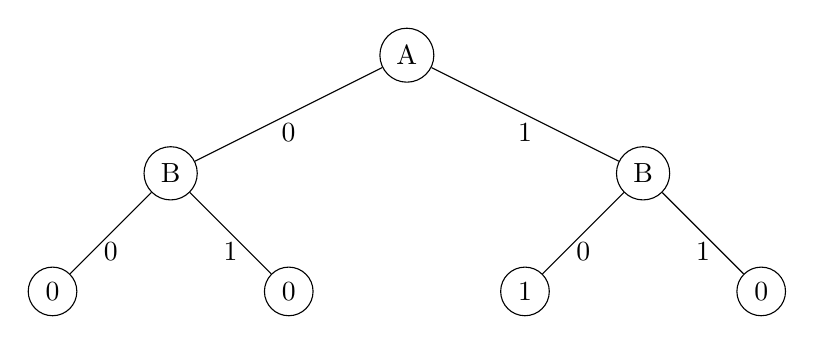
\begin{tikzpicture}
 [level/.style={sibling distance=60mm/#1}]
 
  \node [circle,draw] {A}
    child { node [circle,draw] {B}
      child { node[dummy] {0}
         edge from parent node [below] {0} }
      child { node[dummy] {0}
         edge from parent node [below] {1} }    
      edge from parent node[below] {0} }
    child { node [circle,draw] {B}
      child { node [dummy] {1}
        edge from parent node [below] {0} } 
      child { node [dummy] {0}
         edge from parent node [below] {1} }  
      edge from parent node[below] {1}};
\end{tikzpicture}

When A=0, B returns 0 whether we have the value 0 or 1 for B. We can collapse this B and just return 0.

\begin{tikzpicture}
 [level/.style={sibling distance=60mm/#1}]
 
  \node [circle,draw] {A}
    child { node [circle,draw] {0}
      edge from parent node[below] {0} }
    child { node [circle,draw] {B}
      child { node [dummy] {1}
        edge from parent node [below] {0} } 
      child { node [dummy] {0}
         edge from parent node [below] {1} }  
      edge from parent node[below] {1}};
\end{tikzpicture}

\subsection{Question 5.2}
For the equation $A\vee [B\wedge C]$:

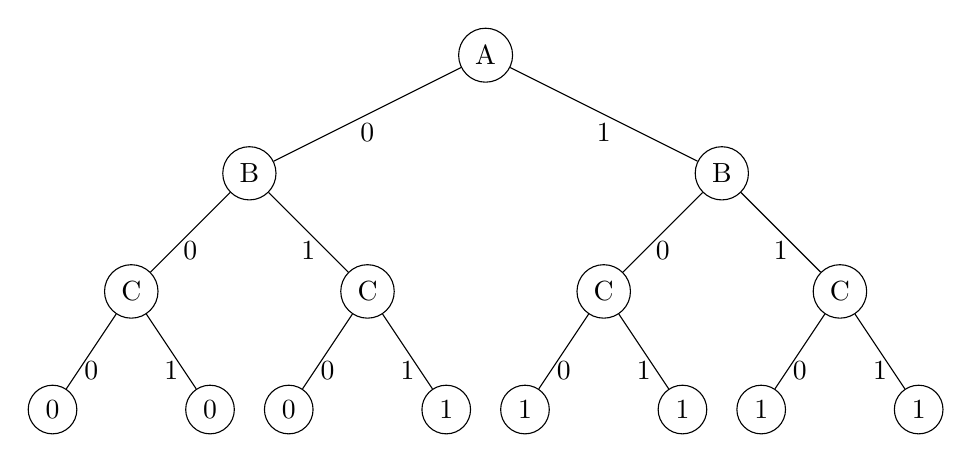
\begin{tikzpicture}
 [level/.style={sibling distance=60mm/#1}]
 
  \node [circle,draw] {A}
    child { node [circle,draw] {B}
      child { node[dummy] {C}
      	 child { node[dummy] {0}
         	edge from parent node [below] {0} }
         child { node[dummy] {0}
         	edge from parent node [below] {1} }
         edge from parent node [below] {0} }
      child { node[dummy] {C}
         child { node[dummy] {0}
         	edge from parent node [below] {0} }
         child { node[dummy] {1}
         	edge from parent node [below] {1} }
         edge from parent node [below] {1} }    
      edge from parent node[below] {0} }
    child { node [circle,draw] {B}
      child { node [dummy] {C}
         child { node[dummy] {1}
         	edge from parent node [below] {0} }
         child { node[dummy] {1}
         	edge from parent node [below] {1} }
         edge from parent node [below] {0} } 
      child { node [dummy] {C}
         child { node[dummy] {1}
         	edge from parent node [below] {0} }
         child { node[dummy] {1}
         	edge from parent node [below] {1} }
         edge from parent node [below] {1} }  
      edge from parent node[below] {1}};
\end{tikzpicture}

When $A = 0$ and $B = 0$, the result is 0 independent form the value of C. This branch will be reduced. Additionally When $A = 1$ the result will be 1 no matter the value of B or C. This will also be reduced. Our new decision tree will be:

\begin{tikzpicture}
 [level/.style={sibling distance=60mm/#1}]
 
  \node [circle,draw] {A}
    child { node [circle,draw] {B}
      child { node[dummy] {0}
         edge from parent node [below] {0} }
      child { node[dummy] {C}
         child { node[dummy] {0}
         	edge from parent node [below] {0} }
         child { node[dummy] {1}
         	edge from parent node [below] {1} }
         edge from parent node [below] {1} }    
      edge from parent node[below] {0} }
    child { node [circle,draw] {1}
      edge from parent node[below] {1}};
\end{tikzpicture}

\subsection{Question 5.3}
For the equation $A \bigoplus B$:

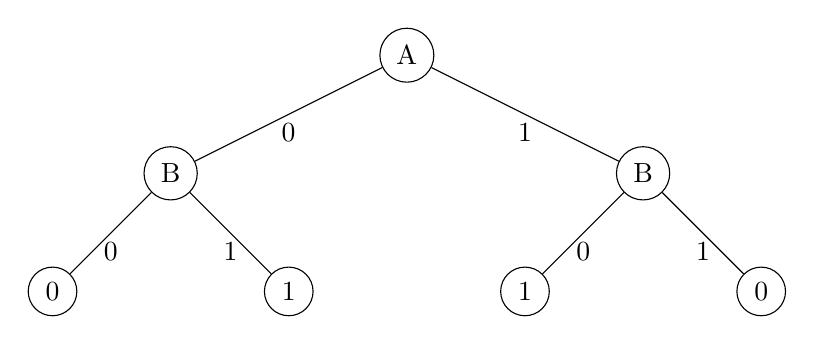
\begin{tikzpicture}
 [level/.style={sibling distance=60mm/#1}]
 
  \node [circle,draw] {A}
    child { node [circle,draw] {B}
      child { node[dummy] {0}
         edge from parent node [below] {0} }
      child { node[dummy] {1}
         edge from parent node [below] {1} }    
      edge from parent node[below] {0} }
    child { node [circle,draw] {B}
      child { node [dummy] {1}
        edge from parent node [below] {0} } 
      child { node [dummy] {0}
         edge from parent node [below] {1} }  
      edge from parent node[below] {1}};
\end{tikzpicture}

This tree cannot be simplified further

\subsection{5.4}
For the equation $[A \wedge B]\vee[C \wedge D]$:

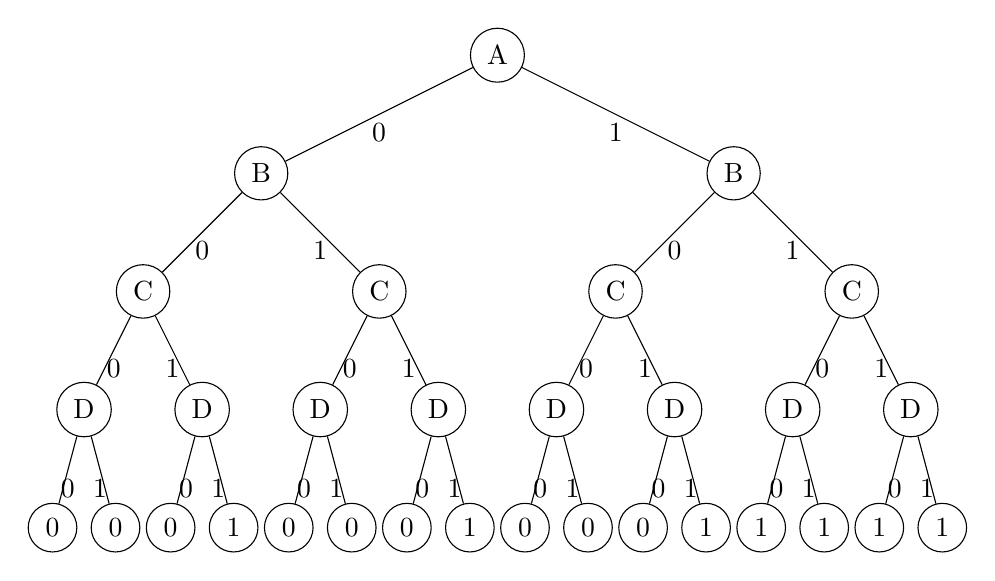
\begin{tikzpicture}
 [level/.style={sibling distance=60mm/#1},
  level 3/.style={sibling distance=15mm},
  level 4/.style={sibling distance=8mm}]
 
  \node [circle,draw] {A}
    child { node [circle,draw] {B}
      child { node[dummy] {C}
      	 child { node[dummy] {D}
      	    child { node[dummy] {0}
               edge from parent node [below] {0} }  
            child { node[dummy] {0}
               edge from parent node [below] {1} }      	         
      	    edge from parent node [below] {0} }
         child { node[dummy] {D}
            child { node[dummy] {0}
               edge from parent node [below] {0} }  
            child { node[dummy] {1}
               edge from parent node [below] {1} } 
         	edge from parent node [below] {1} }
         edge from parent node [below] {0} }
      child { node[dummy] {C}
         child { node[dummy] {D}
            child { node[dummy] {0}
               edge from parent node [below] {0} }  
            child { node[dummy] {0}
               edge from parent node [below] {1} } 
         	edge from parent node [below] {0} }
         child { node[dummy] {D}
            child { node[dummy] {0}
               edge from parent node [below] {0} }  
            child { node[dummy] {1}
               edge from parent node [below] {1} } 
         	edge from parent node [below] {1} }
         edge from parent node [below] {1} }    
      edge from parent node[below] {0} }
    child { node [circle,draw] {B}
      child { node [dummy] {C}
         child { node[dummy] {D}
            child { node[dummy] {0}
               edge from parent node [below] {0} }  
            child { node[dummy] {0}
               edge from parent node [below] {1} } 
         	edge from parent node [below] {0} }
         child { node[dummy] {D}
            child { node[dummy] {0}
               edge from parent node [below] {0} }  
            child { node[dummy] {1}
               edge from parent node [below] {1} } 
         	edge from parent node [below] {1} }
         edge from parent node [below] {0} } 
      child { node [dummy] {C}
         child { node[dummy] {D}
            child { node[dummy] {1}
               edge from parent node [below] {0} }  
            child { node[dummy] {1}
               edge from parent node [below] {1} } 
         	edge from parent node [below] {0} }
         child { node[dummy] {D}
            child { node[dummy] {1}
               edge from parent node [below] {0} }  
            child { node[dummy] {1}
               edge from parent node [below] {1} } 
         	edge from parent node [below] {1} }
         edge from parent node [below] {1} }  
      edge from parent node[below] {1}};
\end{tikzpicture}

Firstly we can see that when A = 0, the trees under B = 0 and B = 1 are identical so they can be combined.

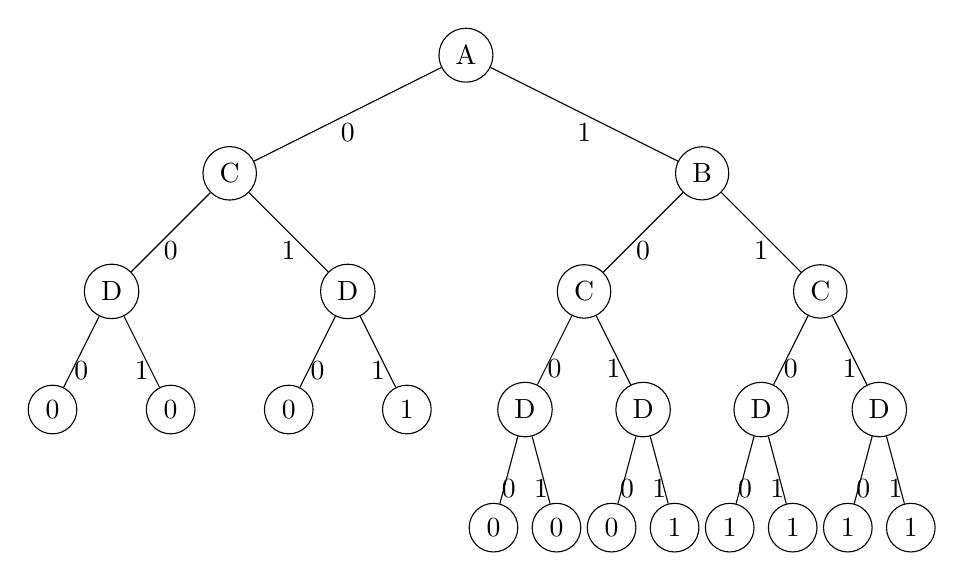
\begin{tikzpicture}
 [level/.style={sibling distance=60mm/#1},
  level 3/.style={sibling distance=15mm},
  level 4/.style={sibling distance=8mm}]
 
  \node [circle,draw] {A}
    child { node[dummy] {C}
         child { node[dummy] {D}
            child { node[dummy] {0}
               edge from parent node [below] {0} }  
            child { node[dummy] {0}
               edge from parent node [below] {1} } 
         	edge from parent node [below] {0} }
         child { node[dummy] {D}
            child { node[dummy] {0}
               edge from parent node [below] {0} }  
            child { node[dummy] {1}
               edge from parent node [below] {1} } 
         	edge from parent node [below] {1} }
         edge from parent node [below] {0} } 
    child { node [circle,draw] {B}
      child { node [dummy] {C}
         child { node[dummy] {D}
            child { node[dummy] {0}
               edge from parent node [below] {0} }  
            child { node[dummy] {0}
               edge from parent node [below] {1} } 
         	edge from parent node [below] {0} }
         child { node[dummy] {D}
            child { node[dummy] {0}
               edge from parent node [below] {0} }  
            child { node[dummy] {1}
               edge from parent node [below] {1} } 
         	edge from parent node [below] {1} }
         edge from parent node [below] {0} } 
      child { node [dummy] {C}
         child { node[dummy] {D}
            child { node[dummy] {1}
               edge from parent node [below] {0} }  
            child { node[dummy] {1}
               edge from parent node [below] {1} } 
         	edge from parent node [below] {0} }
         child { node[dummy] {D}
            child { node[dummy] {1}
               edge from parent node [below] {0} }  
            child { node[dummy] {1}
               edge from parent node [below] {1} } 
         	edge from parent node [below] {1} }
         edge from parent node [below] {1} }  
      edge from parent node[below] {1}};
\end{tikzpicture}

When A = 0 and C = 0, the result is not dependent on D. D collapses to 0. Additionally when A = 1, B = 0 and C = 0 the answer is always 0. That subbranch is also collapsed.

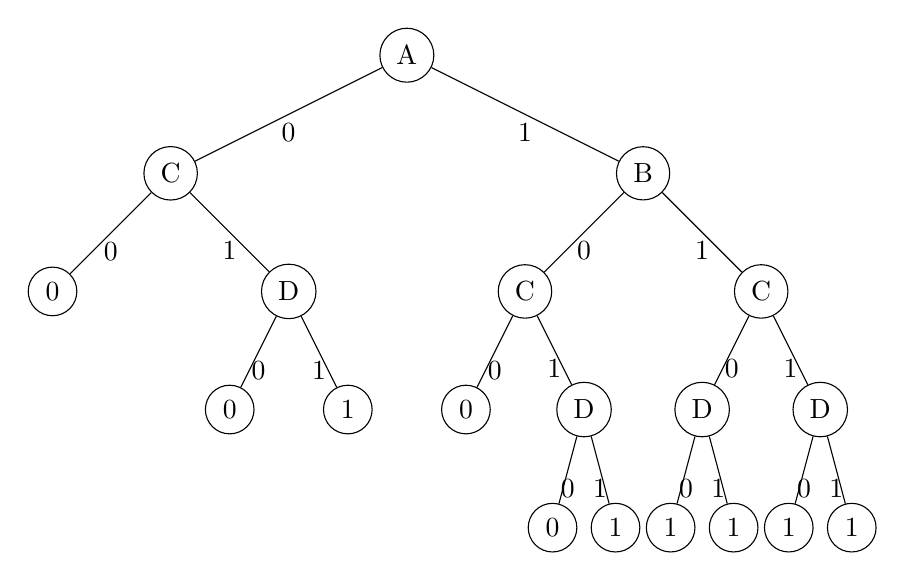
\begin{tikzpicture}
 [level/.style={sibling distance=60mm/#1},
  level 3/.style={sibling distance=15mm},
  level 4/.style={sibling distance=8mm}]
 
  \node [circle,draw] {A}
    child { node[dummy] {C}
         child { node[dummy] {0} 
         	edge from parent node [below] {0} }
         child { node[dummy] {D}
            child { node[dummy] {0}
               edge from parent node [below] {0} }  
            child { node[dummy] {1}
               edge from parent node [below] {1} } 
         	edge from parent node [below] {1} }
         edge from parent node [below] {0} } 
    child { node [circle,draw] {B}
      child { node [dummy] {C}
         child { node[dummy] {0}
         	edge from parent node [below] {0} }
         child { node[dummy] {D}
            child { node[dummy] {0}
               edge from parent node [below] {0} }  
            child { node[dummy] {1}
               edge from parent node [below] {1} } 
         	edge from parent node [below] {1} }
         edge from parent node [below] {0} } 
      child { node [dummy] {C}
         child { node[dummy] {D}
            child { node[dummy] {1}
               edge from parent node [below] {0} }  
            child { node[dummy] {1}
               edge from parent node [below] {1} } 
         	edge from parent node [below] {0} }
         child { node[dummy] {D}
            child { node[dummy] {1}
               edge from parent node [below] {0} }  
            child { node[dummy] {1}
               edge from parent node [below] {1} } 
         	edge from parent node [below] {1} }
         edge from parent node [below] {1} }  
      edge from parent node[below] {1}};
\end{tikzpicture}

Finally when A = 1 and B = 1 the aswer will always be 0 and not dependent on C or D. This branch is collapsed.

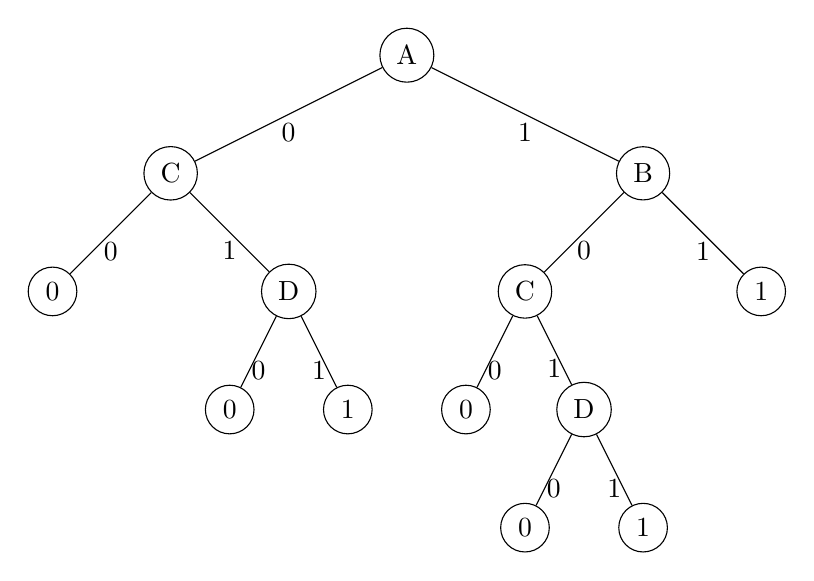
\begin{tikzpicture}
 [level/.style={sibling distance=60mm/#1},
  level 3/.style={sibling distance=15mm},
  level 4/.style={sibling distance=15mm}]
 
  \node [circle,draw] {A}
    child { node[dummy] {C}
         child { node[dummy] {0} 
         	edge from parent node [below] {0} }
         child { node[dummy] {D}
            child { node[dummy] {0}
               edge from parent node [below] {0} }  
            child { node[dummy] {1}
               edge from parent node [below] {1} } 
         	edge from parent node [below] {1} }
         edge from parent node [below] {0} } 
    child { node [circle,draw] {B}
      child { node [dummy] {C}
         child { node[dummy] {0}
         	edge from parent node [below] {0} }
         child { node[dummy] {D}
            child { node[dummy] {0}
               edge from parent node [below] {0} }  
            child { node[dummy] {1}
               edge from parent node [below] {1} } 
         	edge from parent node [below] {1} }
         edge from parent node [below] {0} } 
      child { node [dummy] {1}
         edge from parent node [below] {1} }  
      edge from parent node[below] {1}};
\end{tikzpicture}
\section{Question 6}
\subsection{Question 6a}

Entropy is used to calculate a decision tree in the ID3 algorithm. For a collection of Samples ($S$):

\begin{equation}
\label{ent}
Entropy(S) = \sum_{i=1}^c -p_i log_2p_i
\end{equation}

If we assume we only have 2 outcomes, then we let the number of positive outcomes by p and the number of negative outcomes be n. Then we can write Equation \ref{ent} as

\begin{equation}
Entropy(p,n) = -\frac{p}{p+n}log_2\frac{p}{p+n} - \frac{n}{p+n}log_2\frac{n}{p+n} 
\end{equation}
 
More specifically we compare the gain of different attributes of the sample set. Then create the tree based on the attributes with the greatest gain

\begin{equation}
Gain(S,A) \equiv Entropy(S) - \sum_{v \in Values(A)} \frac{\vert S_v\vert}{\vert S\vert}Entropy(S_v)
\end{equation}

We need to determine $Entropy(S)$

\begin{equation}
\begin{split}
Entropy(p,n) &=  -\frac{p}{p+n}log_2\frac{p}{p+n} - \frac{n}{p+n}log_2\frac{n}{p+n}  \\
           &= -\frac{3}{3+1} log_2\frac{3}{3+1} -\frac{1}{3+1} log_2\frac{1}{3+1} \\
           &= 0.811   \\
\end{split}
\end{equation}

Now we need to determine the gain for the 6 attributes to determine which one will be the root node.

For Sky we have sunny {$p_1=3,n_1=0$) and rainy {$p_2=0,n_2=1$)
\begin{equation}
\begin{split}
\label{sky}
Gain(S,Sky) &= Entropy(S) - \sum_{v \in Values(A)} \frac{\vert S_v\vert}{\vert S\vert}Entropy(S_v) \\
          &= 0.811 - \frac{3}{4} Entropy(S_{Sunny} ) - \frac{1}{4}Entropy(S_{Rainy}) \\
          &= 0.811 - \frac{3}{4} Entropy(3,0) - \frac{1}{4}Entropy(0,1) \\
          &= 0.811 -\frac{3}{4} ( -\frac{3}{3} log_2\frac{3}{3} -\frac{0}{3} log_2\frac{0}{3} ) - \frac{1}{4}(-\frac{0}{1} log_2\frac{0}{1} - \frac{1}{1}log_2\frac{1}{1} ) \\
          &= 0.811 - 0\\
          &= 0.811 \\
\end{split}
\end{equation}

For attribute AirTemp we have warm {$p_1=3,n_1=0$) and cold {$p_2=0,n_2=1$)

\begin{equation}
\begin{split}
\label{airtemp}
Gain(S,AirTemp) &= Entropy(S) - \sum_{v \in Values(A)} \frac{\vert S_v\vert}{\vert S\vert}Entropy(S_v) \\
          &= 0.811 - \frac{3}{4} Entropy(S_{Warm} ) - \frac{1}{4}Entropy(S_{Cold}) \\
          &= 0.811 - \frac{3}{4} Entropy(3,0) - \frac{1}{4}Entropy(0,1) \\
          &= 0.811 -\frac{3}{4} ( -\frac{3}{3} log_2\frac{3}{3} -\frac{0}{3} log_2\frac{0}{3} ) - \frac{1}{4}(-\frac{0}{1} log_2\frac{0}{1} - \frac{1}{1}log_2\frac{1}{1} ) \\
          &= 0.811 - 0\\
          &= 0.811 \\
\end{split}
\end{equation}

For attribute Humidity we have normal {$p_1=1,n_1=0$) and high {$p_1=2,n_2=1$)

\begin{equation}
\begin{split}
\label{humidity}
Gain(S,Humidity) &= Entropy(S) - \sum_{v \in Values(A)} \frac{\vert S_v\vert}{\vert S\vert}Entropy(S_v) \\
          &= 0.811 - \frac{1}{4} Entropy(S_{normal} ) - \frac{3}{4}Entropy(S_{high}) \\
          &= 0.811 - \frac{1}{4} Entropy(1,0) - \frac{3}{4}Entropy(2,1) \\
          &= 0.811 -\frac{1}{4} ( -\frac{1}{1} log_2\frac{1}{1} -\frac{0}{1} log_2\frac{0}{1} ) - \frac{3}{4}(-\frac{2}{3} log_2\frac{2}{3} - \frac{1}{3}log_2\frac{1}{3} ) \\
          &= 0.811 - 0.689\\
          &= 0.123 \\
\end{split}
\end{equation}

For attribute Wind we only have strong {$p_1=3,n_1=1$}

\begin{equation}
\begin{split}
\label{wind}
Gain(S,Wind) &= Entropy(S) - \sum_{v \in Values(A)} \frac{\vert S_v\vert}{\vert S\vert}Entropy(S_v) \\
          &= 0.811 - \frac{4}{4} Entropy(S_{strong} ) \\
          &= 0.811 - \frac{4}{4} Entropy(3,1) \\
          &= 0.811 -\frac{4}{4} ( -\frac{4}{4} log_2\frac{4}{4} -\frac{0}{4} log_2\frac{0}{4} ) \\
          &= 0.811 - 0.811\\
          &= 0.0 \\
\end{split}
\end{equation}

For attribute water we have warm {$p_1=2,n_1=1$) and cold {$p_1=1,n_2=0$)

\begin{equation}
\begin{split}
\label{water}
Gain(S,Water) &= Entropy(S) - \sum_{v \in Values(A)} \frac{\vert S_v\vert}{\vert S\vert}Entropy(S_v) \\
          &= 0.811 - \frac{3}{4} Entropy(S_{warm} ) - \frac{1}{4}Entropy(S_{high}) \\
          &= 0.811 - \frac{3}{4} Entropy(2,1) - \frac{1}{4}Entropy(1,0) \\
          &= 0.811 -\frac{3}{4} ( -\frac{2}{3} log_2\frac{2}{3} -\frac{1}{3} log_2\frac{1}{3} ) - \frac{1}{4}(-\frac{1}{1} log_2\frac{1}{1} - \frac{0}{1}log_2\frac{0}{1} ) \\
          &= 0.811 - 0.689\\
          &= 0.123 \\
\end{split}
\end{equation}

For attribute forecast we have same {$p_1=2,n_1=0$) and change {$p_1=1,n_2=1$)

\begin{equation}
\begin{split}
\label{forcast}
Gain(S,Forecast) &= Entropy(S) - \sum_{v \in Values(A)} \frac{\vert S_v\vert}{\vert S\vert}Entropy(S_v) \\
          &= 0.811 - \frac{2}{4} Entropy(S_{same} ) - \frac{2}{4}Entropy(S_{change}) \\
          &= 0.811 - \frac{2}{4} Entropy(2,0) - \frac{1}{1}Entropy(1,0) \\
          &= 0.811 -\frac{2}{4} ( -\frac{2}{2} log_2\frac{2}{2} -\frac{0}{2} log_2\frac{0}{2} ) - \frac{2}{4}(-\frac{1}{2} log_2\frac{1}{2} - \frac{1}{2}log_2\frac{1}{2} ) \\
          &= 0.811 - 0.5\\
          &= 0.311 \\
\end{split}
\end{equation}

To recap: 
\newline
Gain(Sky) = 0.811 from Equation \ref{sky} \newline
Gain(AirTemp) = 0.811 from Equation \ref{airtemp} \newline
Gain(Humidity) 0.123 from Equation \ref{humidity} \newline
Gain(Wind) = 0 from Equation \ref{wind} \newline
Gain(Water) = 0.123 from Equation \ref{water} \newline
Gain(Forecast) = 0.311 from Equation \ref{forcast} \newline

We find that Sky and Airtemp have the greatest information gain. We could choose either to be the root node. We arbitrarily will choose Sky as the root node. The decision tree so far will look like this:

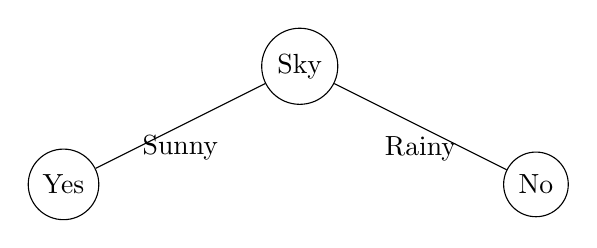
\begin{tikzpicture}
 [level/.style={sibling distance=60mm/#1}]
 
  \node [circle,draw] {Sky}
    child { node [circle,draw] {Yes}    
      edge from parent node[below] {Sunny} }
    child { node [circle,draw] {No}
      edge from parent node[below] {Rainy}};
\end{tikzpicture}


For the leaf node Sky = Sunny, we need to determine the sub-tree.

For Sky = Sunny:

\begin{equation}
\begin{split}
Entropy(S_{Sky=Sunny}) &= Entropy(p,n) \\
                       &= -\frac{p}{p+n}log_2\frac{p}{p+n} - \frac{n}{p+n}log_2\frac{n}{p+n}  \\
                       &= -\frac{3}{3} log_2\frac{3}{3} -\frac{0}{3} log_2\frac{0}{3} \\
                       &= 0   \\
\end{split}
\end{equation}

We need to calculate the information gain for the other attributes when Sky = sunny

For AirTemp we only have warm ($p_1=3,n_1=0$)

\begin{equation}
\begin{split}
Gain(S_{Sky=Sunny},AirTemp) &= 0.0 - \frac{3}{3} Entropy(S_{Sky=Sunny;AirTemp=Warm} )\\
          &= 0.0 - \frac{3}{3} Entropy(3,0) \\
          &= 0.0 - 1( -\frac{3}{3} log_2\frac{3}{3} -\frac{0}{3} log_2\frac{0}{3} )  \\
          &= 0.0 \\
\end{split}
\end{equation}

For Humidity normal ($p_1=1,n_1=0$) and high ($p_2=2,n_2=0$)

\begin{equation}
\begin{split}
Gain(S_{Sky=Sunny},Humidity) &= 0.0 - \frac{1}{3} Entropy(S_{Sky=Sunny;Humidity=Normal} ) \\
&-
    \frac{2}{3}Entropy(S_{Sky=Sunny;Humidity=High})\\
          &= 0.0 - \frac{1}{3} Entropy(1,0) - \frac{2}{3}Entropy(2,0)\\
          &= 0.0 - \frac{1}{3}( -\frac{1}{1} log_2\frac{1}{1} -\frac{0}{1} log_2\frac{0}{1} ) -\frac{2}{3}( -\frac{2}{2}log_2\frac{2}{2} - \frac{0}{2}log_2\frac{0}{2} )  \\
          &= 0.0 \\
\end{split}
\end{equation}

For Wind we only have strong ($p_1=3,n_1=0$)

\begin{equation}
\begin{split}
Gain(S_{Sky=Sunny},Wind) &= 0.0 - \frac{3}{3} Entropy(S_{Sky=Sunny;Wind=Strong} )\\
          &= 0.0 - \frac{3}{3} Entropy(3,0) \\
          &= 0.0 - 1( -\frac{3}{3} log_2\frac{3}{3} -\frac{0}{3} log_2\frac{0}{3} )  \\
          &= 0.0 \\
\end{split}
\end{equation}

For Water we have warm($p_1=2,n_1=0$) and cool($p_2=1,n_2=0$)

\begin{equation}
\begin{split}
Gain(S_{Sky=Sunny},Water) &= 0.0 - \frac{2}{3} Entropy(S_{Sky=Sunny;Water=Warm} ) \\
&-
    \frac{1}{3}Entropy(S_{Sky=Sunny;Water=Cool})\\
          &= 0.0 - \frac{2}{3} Entropy(2,0) - \frac{1}{3}Entropy(1,0)\\
          &= 0.0 - \frac{2}{3}( -\frac{2}{2} log_2\frac{2}{2} -\frac{0}{2} log_2\frac{0}{2} ) -\frac{1}{3}( -\frac{1}{1}log_2\frac{1}{1} - \frac{0}{1}log_2\frac{0}{1} )  \\
          &= 0.0 \\
\end{split}
\end{equation}

For Forecast we have same($p_1=2,n_1=0$) and change($p_2=1,n_2=0$)

\begin{equation}
\begin{split}
Gain(S_{Sky=Sunny},Forecast) &= 0.0 - \frac{2}{3} Entropy(S_{Sky=Sunny;Forecast=Same} ) \\
&-
    \frac{1}{3}Entropy(S_{Sky=Sunny;Forecast=Change})\\
          &= 0.0 - \frac{2}{3} Entropy(2,0) - \frac{1}{3}Entropy(1,0)\\
          &= 0.0 - \frac{2}{3}( -\frac{2}{2} log_2\frac{2}{2} -\frac{0}{2} log_2\frac{0}{2} ) -\frac{1}{3}( -\frac{1}{1}log_2\frac{1}{1} - \frac{0}{1}log_2\frac{0}{1} )  \\
          &= 0.0 \\
\end{split}
\end{equation}

This means that the node Sky = Sunny in our tree will be a leaf node, sice at this node the gain gor all the other attributes are 0.

Next we need to calculate the subtree under the node Sky = Rainy

Starting with  

\begin{equation}
\begin{split}
Entropy(S_{Sky=Rainy}) &= Entropy(p,n) \\
                       &= -\frac{p}{p+n}log_2\frac{p}{p+n} - \frac{n}{p+n}log_2\frac{n}{p+n}  \\
                       &= -\frac{0}{1} log_2\frac{0}{1} -\frac{1}{1} log_2\frac{1}{1} \\
                       &= 0   \\
\end{split}
\end{equation}

For AirTemp we only have cold ($p_1=0,n_1=1$)

\begin{equation}
\begin{split}
Gain(S_{Sky=Rainy},AirTemp) &= 0.0 - \frac{1}{1} Entropy(S_{Sky=Rainy;AirTemp=Cold} )\\
          &= 0.0 - \frac{1}{1} Entropy(0,1) \\
          &= 0.0 - 1( -\frac{0}{1} log_2\frac{0}{1} -\frac{1}{1} log_2\frac{1}{1} )  \\
          &= 0.0 \\
\end{split}
\end{equation}

For Humidity we only have High ($p_1=0,n_1=1$)

\begin{equation}
\begin{split}
Gain(S_{Sky=Rainy},Humidity) &= 0.0 - \frac{1}{1} Entropy(S_{Sky=Rainy;Humidity=High} )\\
          &= 0.0 - \frac{1}{1} Entropy(0,1) \\
          &= 0.0 - 1( -\frac{0}{1} log_2\frac{0}{1} -\frac{1}{1} log_2\frac{1}{1} )  \\
          &= 0.0 \\
\end{split}
\end{equation}

For Wind we only have Strong ($p_1=0,n_1=1$)

\begin{equation}
\begin{split}
Gain(S_{Sky=Rainy},Wind) &= 0.0 - \frac{1}{1} Entropy(S_{Sky=Rainy;Wind=Strong} )\\
          &= 0.0 - \frac{1}{1} Entropy(0,1) \\
          &= 0.0 - 1( -\frac{0}{1} log_2\frac{0}{1} -\frac{1}{1} log_2\frac{1}{1} )  \\
          &= 0.0 \\
\end{split}
\end{equation}

For Water we only have Warm ($p_1=0,n_1=1$)

\begin{equation}
\begin{split}
Gain(S_{Sky=Rainy},Water) &= 0.0 - \frac{1}{1} Entropy(S_{Sky=Rainy;Water=Warm} )\\
          &= 0.0 - \frac{1}{1} Entropy(0,1) \\
          &= 0.0 - 1( -\frac{0}{1} log_2\frac{0}{1} -\frac{1}{1} log_2\frac{1}{1} )  \\
          &= 0.0 \\
\end{split}
\end{equation}

For Forecast we only have Change ($p_1=0,n_1=1$)

\begin{equation}
\begin{split}
Gain(S_{Sky=Rainy},Forecast) &= 0.0 - \frac{1}{1} Entropy(S_{Sky=Rainy;ForeCast=Change} )\\
          &= 0.0 - \frac{1}{1} Entropy(0,1) \\
          &= 0.0 - 1( -\frac{0}{1} log_2\frac{0}{1} -\frac{1}{1} log_2\frac{1}{1} )  \\
          &= 0.0 \\
\end{split}
\end{equation}

This means when Sky = Rainy, the gain from all the other attributes are 0. This means Sky = Rainy is also a leaf node. This means the final tree will be:

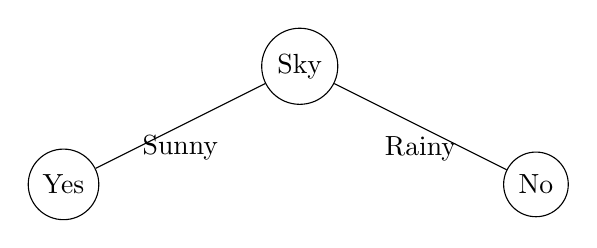
\begin{tikzpicture}
 [level/.style={sibling distance=60mm/#1}]
 
  \node [circle,draw] {Sky}
    child { node [circle,draw] {Yes}    
      edge from parent node[below] {Sunny} }
    child { node [circle,draw] {No}
      edge from parent node[below] {Rainy}};
\end{tikzpicture}

\subsection{Question 6b}
Now we add a new row of training data. We will be recalculating the decision tree. Starting by determining the root node of the tree by comparing the information gain each attribute gives us.

First we need to determine the entropy of S

\begin{equation}
\begin{split}
Entropy(p,n) &=  -\frac{p}{p+n}log_2\frac{p}{p+n} - \frac{n}{p+n}log_2\frac{n}{p+n}  \\
           &= -\frac{3}{3+2} log_2\frac{3}{3+2} -\frac{2}{3+2} log_2\frac{2}{3+2} \\
           &= 0.971   \\
\end{split}
\end{equation}

For the attribute Sky we have Sunny ($p_1=3,n_1=1$) and Rainy ($p_2=0,n_2=1$)

\begin{equation}
\begin{split}
Gain(S,Sky) &= 0.971 -\frac{4}{5} Entropy(S_{Sunny} ) - \frac{1}{5}Entropy(S_{Rainy}) \\
          &= 0.971 - \frac{4}{5} Entropy(3,1) - \frac{1}{5}Entropy(0,1) \\
          &= 0.971 -\frac{4}{5} ( -\frac{3}{4} log_2\frac{3}{4} -\frac{1}{4} log_2\frac{1}{4} ) - \frac{1}{5}(-\frac{0}{1} log_2\frac{0}{1} - \frac{1}{1}log_2\frac{1}{1} ) \\
          &= 0.971 - 0.649\\
          &= 0.322 \\
\end{split}
\end{equation}

For the attribute AirTemp we have Warm ($p_1=3,n_1=1$) and Cold ($p_2=0,n_2=1$)

\begin{equation}
\begin{split}
Gain(S,AirTemp) &= 0.971 - \frac{4}{5} Entropy(S_{Warm} ) - \frac{1}{5}Entropy(S_{Cold}) \\
          &= 0.971 - \frac{4}{5} Entropy(3,1) - \frac{1}{5}Entropy(0,1) \\
          &= 0.971 -\frac{4}{5} ( -\frac{3}{4} log_2\frac{3}{4} -\frac{1}{4} log_2\frac{1}{4} ) - \frac{1}{5}(-\frac{0}{1} log_2\frac{0}{1} - \frac{1}{1}log_2\frac{1}{1} ) \\
          &= 0.971 - 0.649\\
          &= 0.322 \\
\end{split}
\end{equation}

For the attribute Humidity we have Normal ($p_1=1,n_1=1$) and High ($p_2=2,n_2=1$)

\begin{equation}
\begin{split}
Gain(S,Humidity) &= 0.971 - \frac{2}{5} Entropy(S_{Normal} ) - \frac{3}{5}Entropy(S_{High}) \\
          &= 0.971 - \frac{2}{5} Entropy(1,1) - \frac{3}{5}Entropy(2,1) \\
          &= 0.971 -\frac{2}{5} ( -\frac{3}{4} log_2\frac{3}{4} -\frac{1}{4} log_2\frac{1}{4} ) -           \frac{3}{5}(-\frac{0}{1} log_2\frac{0}{1} - \frac{1}{1}log_2\frac{1}{1} ) \\
          &= 0.971 - 0.951\\
          &= 0.020 \\
\end{split}
\end{equation}

For the attribute Wind we have Strong($p_1=3,n_1=1$) and Weak ($p_2=0,n_2=1$)

\begin{equation}
\begin{split}
Gain(S,Wind) &= 0.971 - \frac{4}{5} Entropy(S_{Strong} ) - \frac{1}{5}Entropy(S_{Weak}) \\
          &= 0.971 - \frac{4}{5} Entropy(3,1) - \frac{1}{5}Entropy(0,1) \\
          &= 0.971 -\frac{4}{5} ( -\frac{3}{4} log_2\frac{3}{4} -\frac{1}{4} log_2\frac{1}{4} ) - \frac{1}{5}(-\frac{0}{1} log_2\frac{0}{1} - \frac{1}{1}log_2\frac{1}{1} ) \\
          &= 0.971 - 0.649\\
          &= 0.322 \\
\end{split}
\end{equation}

For the attribute Water we have Warm ($p_1=3,n_1=1$) and Cool ($p_2=1,n_2=0$)

\begin{equation}
\begin{split}
Gain(S,Water) &= 0.971 - \frac{4}{5} Entropy(S_{Warm} ) - \frac{1}{5}Entropy(S_{Cool}) \\
          &= 0.971 - \frac{4}{5} Entropy(3,1) - \frac{1}{5}Entropy(0,1) \\
          &= 0.971 -\frac{4}{5} ( -\frac{3}{4} log_2\frac{3}{4} -\frac{1}{4} log_2\frac{1}{4} ) - \frac{1}{5}(-\frac{1}{1} log_2\frac{1}{1} - \frac{0}{1}log_2\frac{0}{1} ) \\
          &= 0.971 - 0.649\\
          &= 0.322 \\
\end{split}
\end{equation}

For the attribute Forecast we have Same ($p_1=2,n_1=1$) and Change ($p_2=1,n_2=1$)

\begin{equation}
\begin{split}
Gain(S,Forecast) &= 0.971 - \frac{3}{5} Entropy(S_{Same} ) - \frac{2}{5}Entropy(S_{Change}) \\
          &= 0.971 - \frac{3}{5} Entropy(2,1) - \frac{2}{5}Entropy(1,1) \\
          &= 0.971 -\frac{3}{5} ( -\frac{2}{3} log_2\frac{2}{3} -\frac{1}{3} log_2\frac{1}{3} ) - \frac{2}{5}(-\frac{1}{2} log_2\frac{1}{2} - \frac{1}{2}log_2\frac{1}{2} ) \\
          &= 0.971 - 0.951\\
          &= 0.020 \\
\end{split}
\end{equation}

We find that the attributes Sky,AirTemp,Wind and Water all have the highest gain of 0.322. This is already very different from the previous question. For consistency we now choose Sky from these 4 attributes to be our root node. This gives us the following decision tree:

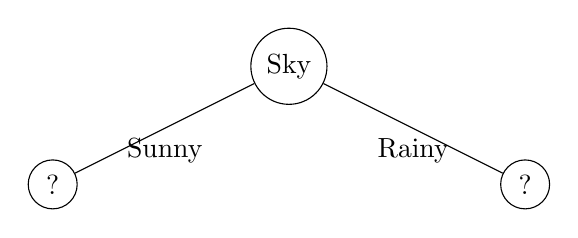
\begin{tikzpicture}
 [level/.style={sibling distance=60mm/#1}]
 
  \node [circle,draw] {Sky}
    child { node [circle,draw] {?}    
      edge from parent node[below] {Sunny} }
    child { node [circle,draw] {?}
      edge from parent node[below] {Rainy}};
\end{tikzpicture}

Continuing with Sky = Sunny, we need to determine the gain of the other attributes so that we can determine the sub-tree. We know that there are 3 positive data rows and one negative for Sky = Sunny:

\begin{equation}
\begin{split}
Entropy(S_{Sky=Sunny}) &= Entropy(p,n) \\
                       &= -\frac{p}{p+n}log_2\frac{p}{p+n} - \frac{n}{p+n}log_2\frac{n}{p+n}  \\
                       &= -\frac{3}{4} log_2\frac{3}{4} -\frac{1}{4} log_2\frac{1}{4} \\
                       &= 0.811   \\
\end{split}
\end{equation}

For attribute AirTemp we have only the value Warm ($p_1=3,n_1=1$)

\begin{equation}
\begin{split}
Gain(S_{Sky=Sunny},AirTemp) &= 0.811 - \frac{3}{3} Entropy(S_{Sky=Sunny;AirTemp=Warm} )\\
          &= 0.811 - \frac{4}{4} Entropy(3,1) \\
          &= 0.811 - 1( -\frac{3}{4} log_2\frac{3}{4} -\frac{1}{4} log_2\frac{1}{4} )  \\
          &= 0.811 - 0.811  \\
          &= 0
\end{split}
\end{equation}

For attribute Humidity we have Normal($p_1=1,n_1=1$) and High ($p_2=2,n_2=0$)

\begin{equation}
\begin{split}
Gain(S_{Sky=Sunny},Humidity) &= 0.811 - \frac{2}{4} Entropy(S_{Sky=Sunny;Humidity=Normal} )\\
                                      &-\frac{2}{4}Entropy(S_{Sky=Sunny;Humidity=High})\\
          &= 0.811 - \frac{2}{4} Entropy(1,1) - \frac{2}{4}Entropy(2,0) \\
          &= 0.811 - \frac{2}{4}( -\frac{1}{2} log_2\frac{1}{2} -\frac{1}{2} log_2\frac{1}{2} ) 
                   - \frac{2}{4}( -\frac{2}{2} log_2\frac{2}{2} -\frac{0}{2} log_2\frac{0}{2} \\
          &= 0.811 - 0.5  \\
          &= 0.311
\end{split}
\end{equation}

For attribute Wind we have Strong($p_1=3,n_1=0$) and Weak ($p_2=0,n_2=1$)

\begin{equation}
\begin{split}
Gain(S_{Sky=Sunny},Wind) &= 0.811 - \frac{3}{4} Entropy(S_{Sky=Sunny;Wind=Strong} )\\
                                      &-\frac{1}{4}Entropy(S_{Sky=Sunny;Wind=Weak})\\
          &= 0.811 - \frac{3}{4} Entropy(3,0) - \frac{1}{4}Entropy(0,1) \\
          &= 0.811 - \frac{3}{4}( -\frac{3}{3} log_2\frac{3}{3} -\frac{0}{3} log_2\frac{0}{3} ) 
                   - \frac{1}{4}( -\frac{0}{1} log_2\frac{0}{1} -\frac{1}{1} log_2\frac{1}{1} \\
          &= 0.811 - 0.0  \\
          &= 0.811
\end{split}
\end{equation}

For attribute Water we have Warm($p_1=2,n_1=1$) and Cool ($p_2=1,n_2=0$)

\begin{equation}
\begin{split}
Gain(S_{Sky=Sunny},Water) &= 0.811 - \frac{3}{4} Entropy(S_{Sky=Sunny;Water=Warm} )\\
                                      &-\frac{1}{4}Entropy(S_{Sky=Sunny;Water=Cool})\\
          &= 0.811 - \frac{3}{4} Entropy(2,1) - \frac{1}{4}Entropy(1,0) \\
          &= 0.811 - \frac{3}{4}( -\frac{2}{3} log_2\frac{2}{3} -\frac{1}{3} log_2\frac{1}{3} ) 
                   - \frac{1}{4}( -\frac{1}{1} log_2\frac{1}{1} -\frac{0}{1} log_2\frac{0}{1} \\
          &= 0.811 - 0.689  \\
          &= 0.123
\end{split}
\end{equation}

For attribute Forecast we have Same($p_1=2,n_1=1$) and Weak ($p_2=1,n_2=0$)

\begin{equation}
\begin{split}
Gain(S_{Sky=Sunny},Forecast) &= 0.811 - \frac{3}{4} Entropy(S_{Sky=Sunny;Forecast=Same} )\\
                                      &-\frac{1}{4}Entropy(S_{Sky=Sunny;Forecast=Change})\\
          &= 0.811 - \frac{3}{4} Entropy(2,1) - \frac{1}{4}Entropy(1,0) \\
          &= 0.811 - \frac{3}{4}( -\frac{2}{3} log_2\frac{2}{3} -\frac{1}{3} log_2\frac{1}{3} ) 
                   - \frac{1}{4}( -\frac{1}{1} log_2\frac{1}{1} -\frac{0}{1} log_2\frac{0}{1} \\
          &= 0.811 - 0.689  \\
          &= 0.123
\end{split}
\end{equation}

Therefore the attribute with the greatest gain when Sky=Sunny is Wind. The Wind attribute will now form our new sub-tree at Sky = Sunny 

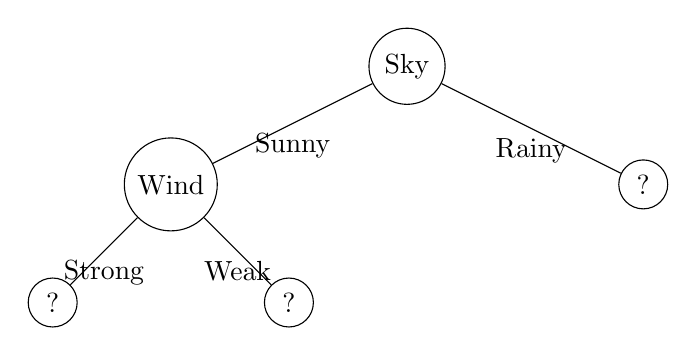
\begin{tikzpicture}
 [level/.style={sibling distance=60mm/#1}]
 
  \node [circle,draw] {Sky}
    child { node [circle,draw] {Wind}  
      child { node[dummy] {?}
         edge from parent node [below] {Strong} }
      child { node[dummy] {?}
         edge from parent node [below] {Weak} }    
      edge from parent node[below] {Sunny} }
    child { node [circle,draw] {?}
      edge from parent node[below] {Rainy}};
\end{tikzpicture}

Now we have to calculate the gains for Sky=Sunny and Wind=Strong. Starting with the Entropy(S) calculation. We can see from the data that there is 3 positive data rows and 0 negative data rows for Sky=Sunny and Wind=Strong 

\begin{equation}
\begin{split}
Entropy(p,n) &=  -\frac{p}{p+n}log_2\frac{p}{p+n} - \frac{n}{p+n}log_2\frac{n}{p+n}  \\
           &= -\frac{3}{3} log_2\frac{3}{3} -\frac{0}{3} log_2\frac{0}{3} \\
           &= 0.0   \\
\end{split}
\end{equation}

For attribute AirTemp we have only the value Warm ($p_1=3,n_1=0$)

\begin{equation}
\begin{split}
Gain(S_{Sky=Sunny;Wind=Strong},AirTemp) &= 0.811 - \frac{3}{3} Entropy(S_{Sky=Sunny;Wind=Strong;AirTemp=Warm} )\\
          &= 0.0 - \frac{3}{3} Entropy(3,0) \\
          &= 0.0 - 1( -\frac{3}{3} log_2\frac{3}{3} -\frac{0}{3} log_2\frac{0}{3} )  \\
          &= 0.0 - 0.0  \\
          &= 0
\end{split}
\end{equation}

For attribute Humidity we have the values Normal ($p_1=1,n_1=0$) and High($p_2=2,n_2=0$)

\begin{equation}
\begin{split}
Gain(S_{Sky=Sunny;Wind=Strong},Humidity) &= 0.0 - \frac{1}{3} Entropy(S_{Sky=Sunny;Wind=Strong,Humidity=Normal} ) \\ &- \frac{2}{3}Entropy(S_{Sky=Sunny;Wind=Strong,Humidity=High}) \\
          &= 0.0 - \frac{1}{3} Entropy(1,0) - \frac{2}{3}Entropy(2,0) \\
          &= 0.0 -\frac{1}{3} ( -\frac{1}{1} log_2\frac{1}{1} -\frac{0}{1} log_2\frac{0}{1} ) - \frac{2}{3}(-\frac{2}{2} log_2\frac{2}{2} - \frac{0}{2}log_2\frac{0}{2} ) \\
          &= 0.0 - 0.0\\
          &= 0 \\
\end{split}
\end{equation}

For attribute Water we have values Cool ($p_1=1,n_1=0$) and Warm($p_2=2,n_2=0$)

\begin{equation}
\begin{split}
Gain(S_{Sky=Sunny;Wind=Strong},Water) &= 0.0 - \frac{1}{3} Entropy(S_{Sky=Sunny;Wind=Strong,Water=Cool} ) \\  &- \frac{2}{3}Entropy(S_{Sky=Sunny;Wind=Strong,Water=Warm}) \\
          &= 0.0 - \frac{1}{3} Entropy(1,0) - \frac{2}{3}Entropy(2,0) \\
          &= 0.0 -\frac{1}{3} ( -\frac{1}{1} log_2\frac{1}{1} -\frac{0}{1} log_2\frac{0}{1} ) - \frac{2}{3}(-\frac{2}{2} log_2\frac{2}{2} - \frac{0}{2}log_2\frac{0}{2} ) \\
          &= 0.0 - 0.0\\
          &= 0 \\
\end{split}
\end{equation}

For attribute Forecast we have values Change ($p_1=1,n_1=0$) and Same($p_2=2,n_2=0$)

\begin{equation}
\begin{split}
Gain(S_{Sky=Sunny;Wind=Strong},Forecast) &= 0.0 - \frac{1}{3} Entropy(S_{Sky=Sunny;Wind=Strong,Forecast=Change} ) \\  &- \frac{2}{3}Entropy(S_{Sky=Sunny;Wind=Strong,Forecast=Same}) \\
          &= 0.0 - \frac{1}{3} Entropy(1,0) - \frac{2}{3}Entropy(2,0) \\
          &= 0.0 -\frac{1}{3} ( -\frac{1}{1} log_2\frac{1}{1} -\frac{0}{1} log_2\frac{0}{1} ) - \frac{2}{3}(-\frac{2}{2} log_2\frac{2}{2} - \frac{0}{2}log_2\frac{0}{2} ) \\
          &= 0.0 - 0.0\\
          &= 0 \\
\end{split}
\end{equation}

We can see that the gains for all the other attributes, when Sky = Sunny and Wind = Strong, are 0. This means that this branch of the tree is complete giving:

 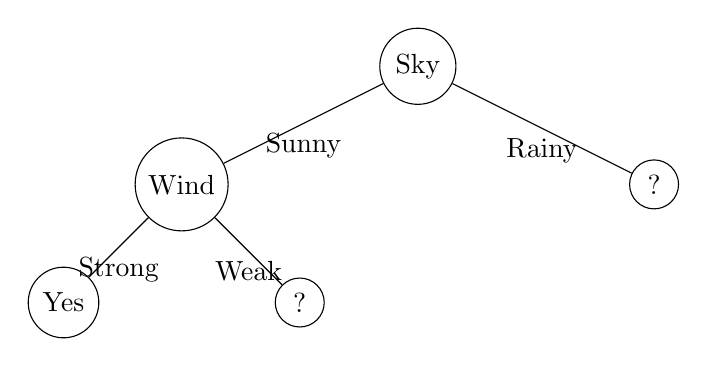
\begin{tikzpicture}
 [level/.style={sibling distance=60mm/#1}]
 
  \node [circle,draw] {Sky}
    child { node [circle,draw] {Wind}  
      child { node[dummy] {Yes}
         edge from parent node [below] {Strong} }
      child { node[dummy] {?}
         edge from parent node [below] {Weak} }    
      edge from parent node[below] {Sunny} }
    child { node [circle,draw] {?}
      edge from parent node[below] {Rainy}};
\end{tikzpicture}

We can classify the leaf node to be yes because all training rows when Sky = Sunny and Wind = Strong has a yes value for EnjoySport.

Now we need to classify the branch Sky = Sunny and Wind = Weak. There are no positive and one negative data rows for Sky = Sunny and Wind = Weak

\begin{equation}
\begin{split}
Entropy(S_{Sky=Sunny,Wind=Weak}) &= Entropy(p,n) \\
                       &= -\frac{p}{p+n}log_2\frac{p}{p+n} - \frac{n}{p+n}log_2\frac{n}{p+n}  \\
                       &= -\frac{0}{1} log_2\frac{0}{1} -\frac{1}{1} log_2\frac{1}{1} \\
                       &= 0   \\
\end{split}
\end{equation}

For the attribute AirTemp we have Warm($p_1=0,n_1=1$)
 
\begin{equation}
\begin{split}
Gain(S_{Sky=Sunny;Wind=Weak},AirTemp) &= 0.0 - \frac{1}{1} Entropy(S_{Sky=Sunny;Wind=Weak;Airtemp=Warm} )\\
          &= 0.0 - \frac{1}{1} Entropy(0,1) \\
          &= 0.0 - \frac{1}{1}( -\frac{0}{1} log_2\frac{0}{1} -\frac{1}{1} log_2\frac{1}{1} ) \\
          &= 0.0 - 0.0  \\
          &= 0
\end{split}
\end{equation}

For the attribute Humidity we have Normal($p_1=0,n_1=1$)
 
\begin{equation}
\begin{split}
Gain(S_{Sky=Sunny;Wind=Weak},Humidity) &= 0.0 - \frac{1}{1} Entropy(S_{Sky=Sunny;Wind=Weak;Humidity=Normal} )\\
          &= 0.0 - \frac{1}{1} Entropy(0,1) \\
          &= 0.0 - \frac{1}{1}( -\frac{0}{1} log_2\frac{0}{1} -\frac{1}{1} log_2\frac{1}{1} ) \\
          &= 0.0 - 0.0  \\
          &= 0
\end{split}
\end{equation}

For the attribute Water we have Warm($p_1=0,n_1=1$)
 
\begin{equation}
\begin{split}
Gain(S_{Sky=Sunny;Wind=Weak},Water) &= 0.0 - \frac{1}{1} Entropy(S_{Sky=Sunny;Wind=Weak;Water=Warm} )\\
          &= 0.0 - \frac{1}{1} Entropy(0,1) \\
          &= 0.0 - \frac{1}{1}( -\frac{0}{1} log_2\frac{0}{1} -\frac{1}{1} log_2\frac{1}{1} ) \\
          &= 0.0 - 0.0  \\
          &= 0
\end{split}
\end{equation}

For the attribute Forecast we have Same($p_1=0,n_1=1$)
 
\begin{equation}
\begin{split}
Gain(S_{Sky=Sunny;Wind=Weak},Forecast) &= 0.0 - \frac{1}{1} Entropy(S_{Sky=Sunny;Wind=Weak;Forecast=Same} )\\
          &= 0.0 - \frac{1}{1} Entropy(0,1) \\
          &= 0.0 - \frac{1}{1}( -\frac{0}{1} log_2\frac{0}{1} -\frac{1}{1} log_2\frac{1}{1} ) \\
          &= 0.0 - 0.0  \\
          &= 0
\end{split}
\end{equation}

Now we can see that the gains of all the attributes, when Sky = Sunny and Wind = Weak, are 0. Additionally we can see that this node would return No, because it is the only option according to our data for Sky = Sunny and Wind = Weak. This gives us:

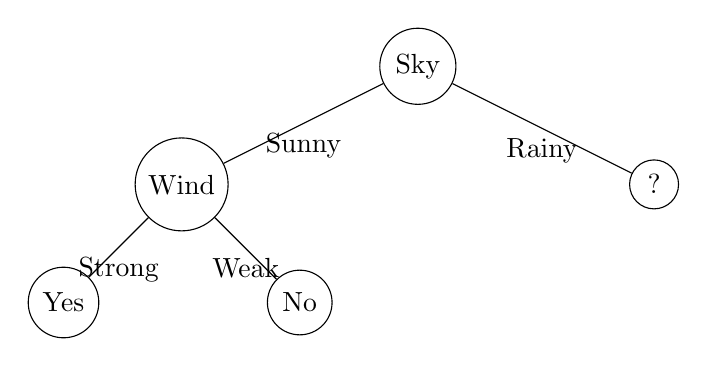
\begin{tikzpicture}
 [level/.style={sibling distance=60mm/#1}]
 
  \node [circle,draw] {Sky}
    child { node [circle,draw] {Wind}  
      child { node[dummy] {Yes}
         edge from parent node [below] {Strong} }
      child { node[dummy] {No}
         edge from parent node [below] {Weak} }    
      edge from parent node[below] {Sunny} }
    child { node [circle,draw] {?}
      edge from parent node[below] {Rainy}};
\end{tikzpicture}

The only branch that still needs classifying is the Sky = Rainy branch. Now we will calculate the gains for the other attributes in this case. For Sky = Rainy, we have only one data row. Which means we have 0 positive and 1 negative data row.

\begin{equation}
\begin{split}
Entropy(S_{Sky=Rainy}) &= Entropy(p,n) \\
                       &= -\frac{p}{p+n}log_2\frac{p}{p+n} - \frac{n}{p+n}log_2\frac{n}{p+n}  \\
                       &= -\frac{0}{1} log_2\frac{0}{1} -\frac{1}{1} log_2\frac{1}{1} \\
                       &= 0   \\
\end{split}
\end{equation}

For the attribute AirTemp we have Cold($p_1=0,n_1=1$)
 
\begin{equation}
\begin{split}
Gain(S_{Sky=Rainy},AirTemp) &= 0.0 - \frac{1}{1} Entropy(S_{Sky=Sunny;AirTemp=Cold} )\\
          &= 0.0 - \frac{1}{1} Entropy(0,1) \\
          &= 0.0 - \frac{1}{1}( -\frac{0}{1} log_2\frac{0}{1} -\frac{1}{1} log_2\frac{1}{1} ) \\
          &= 0.0 - 0.0  \\
          &= 0
\end{split}
\end{equation}

For the attribute Humidity we have High($p_1=0,n_1=1$)
 
\begin{equation}
\begin{split}
Gain(S_{Sky=Rainy},Humidity) &= 0.0 - \frac{1}{1} Entropy(S_{Sky=Sunny;Humidity=High} )\\
          &= 0.0 - \frac{1}{1} Entropy(0,1) \\
          &= 0.0 - \frac{1}{1}( -\frac{0}{1} log_2\frac{0}{1} -\frac{1}{1} log_2\frac{1}{1} ) \\
          &= 0.0 - 0.0  \\
          &= 0
\end{split}
\end{equation}

For the attribute Wind we have Strong($p_1=0,n_1=1$)
 
\begin{equation}
\begin{split}
Gain(S_{Sky=Rainy},Wind) &= 0.0 - \frac{1}{1} Entropy(S_{Sky=Sunny;Wind=Strong} )\\
          &= 0.0 - \frac{1}{1} Entropy(0,1) \\
          &= 0.0 - \frac{1}{1}( -\frac{0}{1} log_2\frac{0}{1} -\frac{1}{1} log_2\frac{1}{1} ) \\
          &= 0.0 - 0.0  \\
          &= 0
\end{split}
\end{equation}

For the attribute Water we have Warm($p_1=0,n_1=1$)
 
\begin{equation}
\begin{split}
Gain(S_{Sky=Rainy},Water) &= 0.0 - \frac{1}{1} Entropy(S_{Sky=Sunny;Water=Warm} )\\
          &= 0.0 - \frac{1}{1} Entropy(0,1) \\
          &= 0.0 - \frac{1}{1}( -\frac{0}{1} log_2\frac{0}{1} -\frac{1}{1} log_2\frac{1}{1} ) \\
          &= 0.0 - 0.0  \\
          &= 0
\end{split}
\end{equation}

For the attribute Forecast we have Change($p_1=0,n_1=1$)
 
\begin{equation}
\begin{split}
Gain(S_{Sky=Rainy},Forecast) &= 0.0 - \frac{1}{1} Entropy(S_{Sky=Sunny;Forecast=Change} )\\
          &= 0.0 - \frac{1}{1} Entropy(0,1) \\
          &= 0.0 - \frac{1}{1}( -\frac{0}{1} log_2\frac{0}{1} -\frac{1}{1} log_2\frac{1}{1} ) \\
          &= 0.0 - 0.0  \\
          &= 0
\end{split}
\end{equation}

We can can see from the gains for the attributes when Sky = Rainy, that we do not create a new sub-tree but make this a leaf node. From the only applicable data row we can see that this node will return No. Therefore the final decision tree will be:

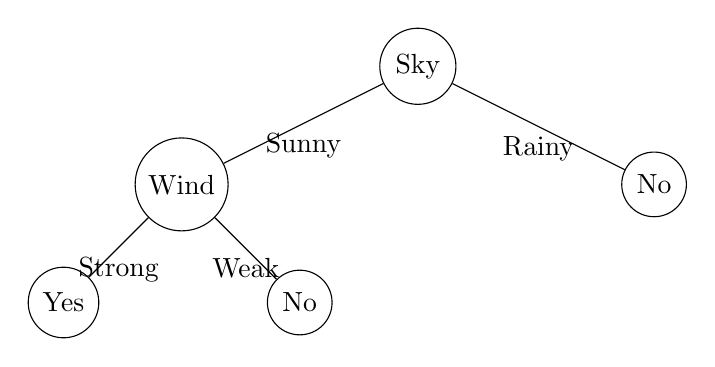
\begin{tikzpicture}
 [level/.style={sibling distance=60mm/#1}]
 
  \node [circle,draw] {Sky}
    child { node [circle,draw] {Wind}  
      child { node[dummy] {Yes}
         edge from parent node [below] {Strong} }
      child { node[dummy] {No}
         edge from parent node [below] {Weak} }    
      edge from parent node[below] {Sunny} }
    child { node [circle,draw] {No}
      edge from parent node[below] {Rainy}};
\end{tikzpicture}


\bibliography{mybib}
\end{document}
